\documentclass[a4paper,12pt]{report}
\usepackage{graphicx}  % For including graphics
\usepackage{hyperref}  % For hyperlinks
\usepackage{listings}  % For code snippets
\usepackage{tocbibind} % For adding ToC to the table of contents
\usepackage{titlesec}  % For customizing titles
\usepackage[ngerman]{babel}
\usepackage{wasysym}
\usepackage{parskip}
\usepackage{bm}


\usepackage{geometry}
\geometry{
    top=1in,
    left=1in,
    right=1in,
    bottom=1in
}


\titleformat{\chapter}[block]   % Set chapter format to block style (both on same line)
{\normalfont\huge\bfseries}     % Format for the chapter number and title
{\thechapter}                   % Shows the chapter number followed by a dot
{0.5em}                         % Space between the chapter number and title
{}                              % Formatting for the chapter title (leave empty)

\renewcommand{\contentsname}{Inhaltsverzeichnis}
\renewcommand{\listtablename}{Tabellenverzeichnis}
\renewcommand{\listfigurename}{Abbildungsverzeichnis}
\renewcommand{\lstlistlistingname}{Code-Ausschnitte}
\renewcommand{\abstractname}{Zusammenfassung}
\renewcommand{\chaptername}{Kapitel}

\begin{document}

% Title Page
    \begin{titlepage}
        \centering
        \textit{Berner Fachhochschule}\\[0.2em]
        \textit{BTI3031 Project 1}
        \vfill
        {\huge \textbf{AI-Aided Caches-n-Logs Monitoring-n-Wiping Daemon}}\\[4em]
        {\large Luca Scherer, Janic Scherer, Luca Ammann }\\[0.5em]
        \begin{tabular}{ll}
            \textbf{Betreuer:}\hspace{0.5em}Dr. Simon Kramer \\
        \end{tabular}

        \vfill
        \textit{\today}
    \end{titlepage}

% Abstract
    \begin{abstract}
        \ldots
    \end{abstract}

% Table of Contents
    \tableofcontents
    \listoftables
    \listoffigures
    \lstlistoflistings

% Main Content


    \chapter{Einleitung}


    \section{Ausgangssituation}


    \section{Projektziel}


    \section{Prioritäten}


    \chapter{Spezifikation}

    \newpage


    \section{Systemabgrenzung}

    \subsection{Systemumgebung}

    \subsubsection{Komponenten}


    \begin{figure}[h]
        \centering
        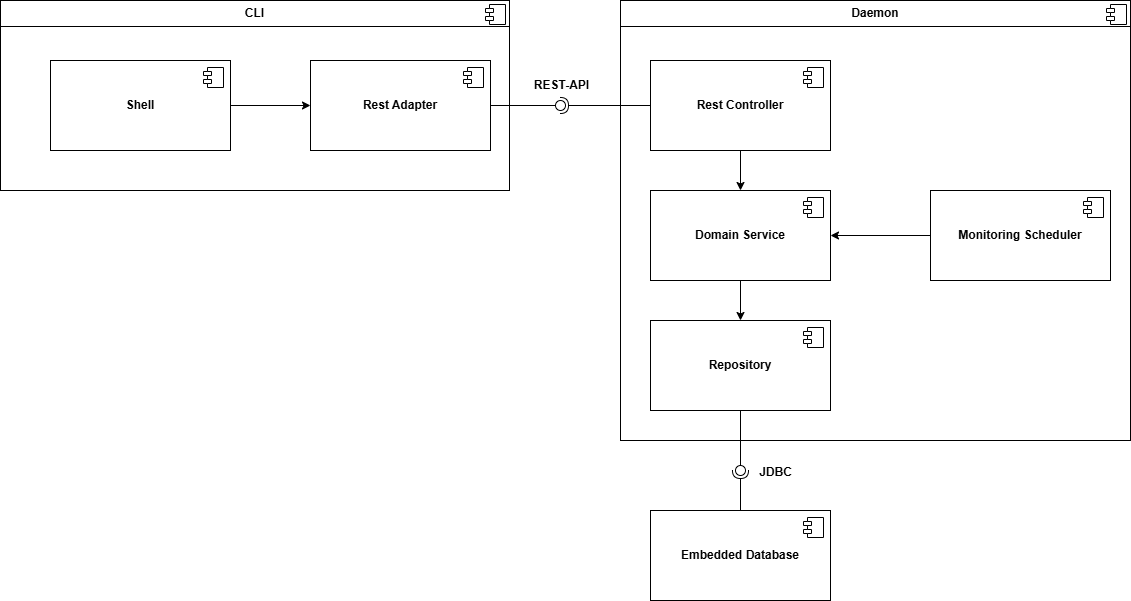
\includegraphics[width=1\textwidth]{assets/comp-diag-tracesentry-v2}
        \caption{UML Komponentendiagramm}
        \label{fig:comp-diag}
    \end{figure}

    \textnormal{Das System besteht aus zwei Hauptkomponenten, welche als eigene Laufzeiteinheiten ausgeführt werden.
    Die CLI wird ad hoc gestartet und dient als Benutzerschnittstelle.
    Der Daemon läuft nach dem Start im Hintergrund und führt periodisch Befehle aus. Ausserdem stellt er der
    CLI eine REST-Schnittstelle zur Verfügung.
    Ein eingebettetes Datenbanksystem speichert die Applikationsdaten.}

    \begin{table}[h!]
        \centering
        \setlength{\leftmargini}{0.4cm}
        \begin{tabular}{|p{2.5cm}|p{5.5cm}|p{3cm}|}
            \hline
            \textbf                       & \textbf{Zweck}                                                    & \textbf{Technologien (primär)} \\
            \hline
            \textbf{Shell}                & {Stellt eine Kommandozeilen-Benutzerschnittstelle zur Verfügung.} & Java, Spring (Shell)           \\
            \hline
            \textbf{Rest Adapter}         & {Stellt den Zugang zur REST-Schnittstelle zur Verfügung}          & Java, Spring (Web)             \\
            \hline
            \textbf{Rest Controller}      & Implementiert die Endpunkte der REST-Schnittstelle                & Java, Spring (Web)             \\
            \hline
            \textbf{Domain Service}       & Applikationslogik                                                 & Java, Spring                   \\
            \hline
            \textbf{Monitoring Scheduler} & Führt Monitoring-Funktionen periodisch aus                        & Java, Spring                   \\
            \hline
            \textbf{Repository}           & Stellt den Zugang zu den persisiterten Daten zur Verfüfung        & Java, Spring (Data)            \\
            \hline
            \textbf{Embedded Database}    & Speichert Applikationsdaten                                       & SQLite                         \\
            \hline
        \end{tabular}
        \caption{Beschreibung der Komponenten}\label{tab:table3}
    \end{table}

    \newpage

    \subsection{Prozessumgebung}

    \newpage


    \section{Anforderungen}
    Die Anforderungen für den AI-Aided Caches-n-Logs Monitoring-n-Wiping Demon ergaben sich aus dem Projekt Proposal sowie einem initialen Termin mit Herr Kramer.

    \subsection{Funktionale Anforderungen}

    Alle funktionalen Anforderungen werden in Form von User Stories im Scrum Product Backlog geführt. Dieser wird laufend erweitert beziehungsweise konkretisiert. Eine User Story gilt erst als abgeschlossen, sobald alle dazugehörende Akzeptanzkriterien erfüllt sind. Folgende funktionale Anforderungen wurden definiert und in User Stories inkl. Akzeptanzkriterien abgebildet:
    \begin{itemize}
        \item Das System findet jegliche Log- oder Cache-Dateien, welche sich in einem angegebenen Verzeichnis befinden. Dabei werden auch alle Unterverzeichnisse berücksichtigt.
        \item Das System durchsucht periodisch angegebene Verzeichnisse inkl. Unterverzeichnisse nach Log- oder Cache-Dateien.
        \item Das System erstellt periodisch sogenannte Snapshots der gefundenen Dateien, um diese später miteinerander zu vergleichen.
        \item Das System identifiziert veränderte Dateien anhand der periodisch erstellten Snapshots.
        \item Das System kann den Verwendungszweck von angegebenen Dateien erkennen und nach folgenden Merkalen kategorisieren oder bewerten:
        \begin{itemize}
            \item Dateityp
            \item Verwendungszweck
            \item Schädlichkeit
            \item Leer- bzw. löschbar
        \end{itemize}
        \item Das System kann angegebene Dateien, nach einer Bestätigung des Benutzers leeren oder löschen.
    \end{itemize}
    TODO: Backlog einbinden/beschreiben

    \newpage

    \subsection{Grenz- und Vorbedingungen}
    Im Scrum Product Backlog werden nichtfunktionalen Anforderungen bzw. Grenz- oder Vorbedingungen nicht explizit als User Story geführt. Aus dem Projekt-Proposal und dem initialen Termin ergaben sich nachfolgende nichtfunktionale Anforderungen.
    Diese beeinflussten massgeblich die Architektur des Systems. Keine User Story darf eine oder mehrere nichtfunktionale Anforderungen verletzten, was durch die Definition of Done sichergestellt und laufend geprüft wird.

    \begin{table}[h!]
        \centering
        \setlength{\leftmargini}{0.4cm}
        \begin{tabular}{|c|p{10cm}|}
            \hline
            \textbf{ID}           & NFR-001                                                                                            \\ \hline
            \textbf{Anforderung}  & Hintergrundprozess mit periodischem Task (deamon)                                                  \\ \hline
            \textbf{Beschreibung} & Das System muss einen Hintergrundprozess implementieren, der periodisch Aktionen durchführen kann. \\ \hline
            \textbf{Akzeptanzkriterien} &
            \begin{itemize}
                \item Nach dem Start des Prozesses, ist dieser für den Benutzer nicht mehr ersichtlich.
                \item Der Hintergrundprozess ist erweiterbar, sodass dieser periodisch und autonom Aktionen durchführen kann.
            \end{itemize}
            \\ \hline
        \end{tabular}
        \caption{Nichtfunktionale Anforderung NFR-001}\label{tab:nfr-1}
    \end{table}

    \begin{table}[h!]
        \centering
        \setlength{\leftmargini}{0.4cm}
        \begin{tabular}{|c|p{10cm}|}
            \hline
            \textbf{ID}           & NFR-002                                                              \\ \hline
            \textbf{Anforderung}  & Benutzerschnittstelle via Konsole (CLI)                              \\ \hline
            \textbf{Beschreibung} & Mit dem laufenden deamon soll via Konsole interagiert werden können. \\ \hline
            \textbf{Akzeptanzkriterien} &
            \begin{itemize}
                \item Der deamon kann via CLI gestartet werden.
                \item Alle Konfigurationen und Aktionen des deamon sind via CLI verfügbar
            \end{itemize}
            \\ \hline
        \end{tabular}
        \caption{Nichtfunktionale Anforderung NFR-002}\label{tab:table4}
    \end{table}

    \begin{table}[h!]
        \centering
        \setlength{\leftmargini}{0.4cm}
        \begin{tabular}{|c|p{10cm}|}
            \hline
            \textbf{ID}           & NFR-003                                                                 \\ \hline
            \textbf{Anforderung}  & Systemunabhängigkeit                                                    \\ \hline
            \textbf{Beschreibung} & Lauffähigkeit mit vollem Funktionsumfang auf gängigen Betriebssystemen. \\ \hline
            \textbf{Akzeptanzkriterien} &
            \begin{itemize}
                \item Hintergrundprozess sowie Konsolenschnittstelle sind auf allen gängigen Betriebssystemen lauffähig und mit vollem Funktionsumfang verwendbar.
                \item Neuimplementierte Features werden auf aktuellen Versionen von Windows, Linux (Ubuntu) und MacOS getestet.
            \end{itemize}
            \\ \hline
        \end{tabular}
        \caption{Nichtfunktionale Anforderung NFR-003}\label{tab:table5}
    \end{table}

    \begin{table}[h!]
        \centering
        \setlength{\leftmargini}{0.4cm}
        \begin{tabular}{|c|p{10cm}|}
            \hline
            \textbf{ID}           & NFR-004                                        \\ \hline
            \textbf{Anforderung}  & Codequalität \& erweiterbare Architektur       \\ \hline
            \textbf{Beschreibung} & Minimaler, modularer und selbserklärender Code \\ \hline
            \textbf{Akzeptanzkriterien} &
            \begin{itemize}
                \item Die Architketur wird so aufgebaut, dass neue Features problemlos ergänzt werden können. (z.B. GUI)
                \item Tests gemäss Testkonzept.
                \item Statische Analysen zeigen keine schwerwiegenden verstösse gegen Linting-Regeln.
                \item Anwendungen von gängigen Design-Prinzipen vie SOLID, DRY, KISS etc.
                \item Für jede Codeerweiterung wird eine Codereview durch einen zweiten Entwickler vorgenommen.
            \end{itemize}
            \\ \hline
        \end{tabular}
        \caption{Nichtfunktionale Anforderung NFR-004}\label{tab:table6}
    \end{table}

    \clearpage

    \subsection{Testkonzept}

    \subsubsection{Ziel des Testkonzepts}
    \begin{itemize}
        \item Sicherstellen, dass das gesamte System stabil läuft und seine Hauptfunktionen zuverlässig verfügbar sind.
        \item Minimales Testing-Setup, das nur dort Unit-Tests verwendet, wo es Sinn ergibt (z. B. kritische Algorithmen), um den Entwicklungsaufwand gering zu halten.
        \item Fokus auf Integrationstests und funktionale Tests zur Überprüfung der gesamten Systemfunktionalität.
        \item Klare Definition, welche Tests während der Entwicklung (Teil einer User Story) umgesetzt werden sollen.
    \end{itemize}

    \subsubsection{Testarten und Testabdeckung}
    \begin{itemize}
        \item \textbf{Unit-Tests}: Nur für kritische, isolierbare Logiken wie:
        \begin{itemize}
            \item \textbf{Hash-Algorithmen}: Test der Konsistenz und Korrektheit, insbesondere, wenn Hashes fürs Verzeichnis Monitoring verwendet werden.
            \item \textbf{File-Suche}: Suchalgorithemen für Log- oder Cache-Dateien.
        \end{itemize}
        \item \textbf{Integrationstests}: Testen der Zusammenarbeit mehrerer Komponenten.
        \begin{itemize}
            \item \textbf{CLI-Befehle}: Überprüfen, dass die CLI-Kommandos (\texttt{run}, \texttt{search}) korrekt ausgeführt werden und die erwarteten Parameter validieren.
            \item \textbf{REST-HTTP-Anfragen}: Testen, ob alle HTTP-Schnittstellen korrekt reagieren. (Happy- sowie Exception-Paths)
        \end{itemize}
        \item \textbf{End-to-End Tests}: Fokus auf End-to-End-Szenarien zur Validierung der zentralen Funktionalität.
    \end{itemize}

    \subsubsection{Test-Setup und -Konfiguration}
    \begin{itemize}
        \item \textbf{Mocking von Ressourcen}: Verwenden von Mocks für Datenbank- und Dateisystemzugriffe in den Unit-Tests, um sie isoliert zu halten.
        \item \textbf{Testumgebung}: Erstellen einer dedizierten Test-DB und eines Testverzeichnisses.
        \item \textbf{Automatisierte Testausführung}: Integration der Tests in die CI/CD-Pipeline, um sicherzustellen, dass das System stabil bleibt.
    \end{itemize}

    \clearpage


    \section{Usability}\label{sec:usability}

    \subsection{Personas}\label{subsec:personas}

    \subsubsection{Thomas}

    \begin{figure}[h]
        \centering
        
\includegraphics[width=0.6\textwidth]{assets/persona1}
        \caption{Thomas \footnote}
        \label{fig:persona-1}
    \end{figure}


    Thomas ist ein 35-Jähriger Berufsschullehrer, der Informatiker und Elektroniker unterrichtet.
    Für seine Schüler unterrichtet er unter anderem auch
    Systemadministration und IT-Sicherheit.
    Thomas ist sehr interessiert an neuen Technologien und probiert gerne neue Software aus.
    Daher stellt er sich die Frage, warum so viele Log- und Cache-Dateien auf seinem Rechner sind, ob diese alle
    ihre Daseinsberechtigung haben und auch ob das Lesen und Schreiben dieser Dateien nicht ein Sicherheitsrisiko
    darstellt.
    Thomas ist ein sehr erfahrener Benutzer und hat keine Probleme mit der Kommandozeile.

    \begin{table}[h!]
        \centering
        \setlength{\leftmargini}{0.4cm}
        \begin{tabular}{|p{2.5cm}|p{7cm}|}
            \hline
            \textbf Aufgaben    & KnowHow stärken (in Bezug auf seine Lehrtätigkeiten)                      \\
            \hline
            \textbf Ziele       & Veränderungen beobachten können und diese überprüfen lassen               \\
            \hline
            \textbf Wünsche     & Intuitive Benutzerschnittstelle                                           \\
            \hline
            \textbf Hindernisse & Trotz Erfahrung in der Informatik, sind teilweise Wissenslücken vorhanden \\
            \hline
        \end{tabular}
        \label{tab:table7}
    \end{table}

    \footnotetext{\url{https://www.pexels.com/de-de/foto/mann-arbeiten-tippen-pc-16129724/}.}


    \newpage


    \section{Usability}

    \subsection{Personas}

    \subsection{Storyboard}

    \subsection{UX-Prototyping}


    \chapter{Implementierung}

    \subsection{Performanz und Optimierung}
    \subsubsection{Komplexität}

    Unser System ist von Grund auf auf Effizienz und Performanz ausgelegt, der Hashbaum als zentrale Datenstruktur ermöglicht dies.
    Die Datenmenge mit der ein Benutzer arbeitet, kann sehr gross werden, daher ist es wichtig, dass die Skalierbarkeit des Systems gewährleistet ist.
    Daher ist eine Analyse der Komplexität der verschiedenen Operationen angebracht.
    \\
    Jeder Ordner und jede Datei wird als Knoten im Hashbaum repräsentiert.
    Die Wurzel des Hashbaums repräsentiert den zu überwachenden Pfad.
    Dateien sind stets Blätter.\newline
    Sei $n$ die Anzahl der Knoten im Verzeichnis des zu überwachenden Pfades.

    \paragraph{Bau}
    Der Baualgorithmus besucht rekursiv alle Dateien und Ordner im zu überwachenden Pfad,
    was einer Komplexität von $O(n)$ für das Traversieren entspricht.
    Das Hashen eines Ordners mit $k$ Kindern setzt eine Iteration über alle Kinder voraus, was einer Komplexität von $O(k)$ entspricht.
    Das Hashen eines Blattes (Datei) ist abhängig von der Grösse $s$ der Datei und hat eine Komplexität von $O(s)$.
    \\\\
    Die Gesamtkomplexität des Bauens des Hashbaums beträgt also \boldsymbol{$O(n * s)$}
    Hier ist $s$ die durchschnittliche Dateigrösse. $k$ ist implizit in $n$ enthalten.

    \paragraph{Linearisierung}
    Es gibt Fälle, in denen der Hashbaum linearisiert wird, um z.B.\ die Java Stream API zu verwenden oder direkt alle Knoten miteinander zu persisitieren.
    Es werden für alle Knoten die Referenzen in einer Liste gespeichert, was einer Komplexität von  \boldsymbol{$O(n)$} entspricht.


    \subsubsection{Caching}
    Bei den folgenden zwei Fällen haben wir uns überlegt, ob es sich lohnen würde, ein Caching einzubauen,
    haben uns dann aber aus den aufgelisteten Gründen dagegen entschieden.

    \begin{enumerate}
        \item Pro MonitoredPath könnte man immer den letzten gebauten MerkleTree cachen, um beim nächsten Snapshot
        direkt mit dem gecachten Baum verlgeichen zu können, ohne diesen wieder aus der Datenbank laden zu müssen.
        \begin{itemize}
            \item Caching macht nur Sinn wenn mehrmals die gleichen Daten gelesen werden.
            Da aber der MerkleTree vom letzten Snapshot nur einmal wiederverwendet wird (beim Vergleichen mit dem Neuen), macht dies hier keinen Sinn.
            \item Kein sich lohnender Mehrwert an Performance gegenüber dem Laden aus der DB, da die DB lokal ist und die Query
            eine tiefe Komplexität hat, kann bereits effizient auf die Daten zugegriffen werden.
        \end{itemize}
        \item Pro MonitoredPath eine geordnete Liste nur mit den Änderungen von jedem Snapshot, damit diese bei der Abfrage
        direkt aus dem Memory zurückgegeben werden können und nicht noch die DB abgefragt werden muss.
        \begin{itemize}
            \item Auch hier wird keine sich lohnende Performance-Steigerung erwartet, denn auch wenn die Daten schon in Memory wären
            braucht es für die zusammengefasste Response der abgefragten Vergleiche trotzdem noch Logik,
            welche auch mit einem Query auf die lokale DB implementiert werden kann und so kein grosser Gewinn daraus resultiert.
        \end{itemize}
    \end{enumerate}

    \subsubsection{Indexing}
    Anhand der folgenden Punkte wurde entschieden, ob/für welche Attribute in der DB ein SQL-Index sinnvoll wäre.

    Index sinnvoll:
    \begin{itemize}
        \item Attribut hat viele verschiedene Werte
        \item Attribut hat wenige/keine null-Werte
        \item Attribut wird oft in einer SQL WHERE oder JOIN Abfrage genutzt
    \end{itemize}

    Index nicht sinnvoll:
    \begin{itemize}
        \item kleine Tabelle
        \item Attribut wird oft manipuliert
    \end{itemize}

    So wurde entschieden die folgenden Attribute zu indexieren:
    \begin{itemize}
        \item \verb|snapshot_node.snapshot_id|
        \item \verb|snapshot_node.has_changed|
        \item \verb|snapshot_node.deleted_in_next_snapshot|
    \end{itemize}

    \section{Architektur}

    \subsection{Architekturentscheid}
    In diesem Abschnitt soll erläutert werden, was wir uns für Gedanken bezüglich der Architektur gemacht haben
    und für was wir uns schlussendlich aus welchen Gründen entschieden haben.

            {\large\bfseries Daemon}

    Als erstes war uns aus den Anforderungen klar, dass wir einen Daemon brauchen, also ein Programm, welches immer im
    Hintergrund (seit Start des Computers) laufen soll.
    Also muss das bereits ein eigenständiges Programm sein, das z.B. beim Systemstart (Autostart bei Windows) ausgeführt werden kann.

            {\large\bfseries Database}

    Als nächstes gibt es die Anforderung, dass Pfad-Analysen zu einem späteren Zeitpunkt verglichen werden können sollen.
    So war für uns auch klar, dass wir eine Datenbank (DBMS) brauchen.
    Dazu haben wir verschiedene Varianten:

    \textbf{1. In-Memory}
    In diesem Fall würde die Datenbank mit dem Start des Programms mitinitialisiert und beim Beenden des Programms auch wieder gelöscht.
    Das bedeutet die Datenbank lebt nur während der Laufzeit des Programms und braucht auch den Speicher des Programms mit.

    \textbf{Begründung zur Variante In-Memory} Diese kommt für uns nicht in Frage, da wir die Analysen auch über die Laufzeit des Daemons hinaus persistieren möchten.
    Damit der Anwender beispielsweise auch nach einem Neustart noch Zugriff auf seine früheren Datei-Analysen hat.

    \textbf{2. Embedded}
    Hier wird die Datenbank in Form von Files innerhalb des Programms (Programm-Ressourcen) mitgeliefert und bleibt
    somit persistent solange es nicht gelöscht wird im Verzeichnis des Programms.

    \textbf{Vorteile}
    \begin{itemize}
        \item Braucht keine externe Infrastruktur
        \item Offline-Verfügbarkeit
        \item Performance
    \end{itemize}

    \textbf{Nachteile}
    \begin{itemize}
        \item Datenverlust bei einem Problem des Anwender-Systems
    \end{itemize}

    \textbf{Begründung zur Variante Embedded} Diese Variante passt für unseren Use-Case am Besten, da wir nur ein kleines System entwickeln.
    Dadurch brauchen wir keine grosse Kapazität an Speicher.
    Die Datenbank ist ebenso einfach und schnell eingerichtet und benötigt keine weitere Infrastruktur.
    Die Verantwortung der Datenbank liegt somit nicht bei uns, sondern beim Anwender.
    Dazu streben wir an, unser System vorallem offline zu betreiben.

    \textbf{3. Remote}
    Hier läuft die Datenbank auf einem externen System und ist über das Netzwerk für unser Programm erreichbar.
    Somit persistent solange auf dem externen System nichts gelöscht wird oder das System nicht beschädigt wird.

    \textbf{Vorteile}
    \begin{itemize}
        \item Datensicherheit
        \item Kapazität
    \end{itemize}

    \textbf{Nachteile}
    \begin{itemize}
        \item Nicht erreichbar ohne Netzwerkverbindung
        \item Braucht externe Infrastruktur (Kosten, Aufwand)
    \end{itemize}

    \textbf{Begründung zur Variante Remote} Diese Variante bringt für uns keinen Mehrwert gegenüber der Embedded-Variante.
    Es wäre eher nur Mehraufwand, der sich aktuell nicht lohnt.

            {\large\bfseries TaskScheduler}

    Für die Anforderung, dass periodisch Dateipfade analysiert werden sollen, war für uns klar dass wir dafür so etwas wie einen
    Task-Scheduler brauchen.
    Und da wir den Daemon genau für das haben ist auch klar, dass diese Tasks am einfachsten über den Daemon gesteuert werden können.
    So ist es auch für die Kommunikation einfacher, da die Resultate der Analyse-Tasks direkt wieder zum Daemon zurückkommuniziert werden können
    und so auch einfach weiterverarbeitet werden können, was vor allem das Speichern in die Datenbank betrifft.

            {\large\bfseries Anwender-Schnittstelle}

    Als Nächstes müssen wir dem Anwender natürlich noch eine Schnittstelle anbieten, über die er Anweisungen/Funktionen von unserem System
    aufrufen kann.
    Dafür gibt es folgende Möglichkeiten:

    \textbf{1. CLI}
    Diese Variante bietet dem Anwender an, über das Kommandozeilen-Interface das System anzuwenden und somit über
    Text-Input auch wieder Text-Output als Resultat zu erhalten.

    \textbf{Vorteile}
    \begin{itemize}
        \item Simpel/Schlicht
    \end{itemize}

    \textbf{Nachteile}
    \begin{itemize}
        \item Schwierigere Anwendung für Anfänger
    \end{itemize}

    \textbf{Begründung CLI} Auch hier haben wir entschieden eine möglichst simple Variante mit geringem initialen Aufwand zu wählen.
    In erster Linie geht es um die Funktionalität, welche auch problemlos mit der CLI-Variante umgesetzt werden kann.
    In der Zukunft können immernoch weitere Schnittstellen hinzugefügt werden, um das System benutzerfreundlicher zu gestalten.

    \textbf{2. GUI}
    Bei der GUI-Variante würde es ein neues Fenster geben z.B. über den Browser oder als Desktop-Applikation,
    worüber der Anwender das System benutzen könnte.
    So wäre es zu Beginn sicherlich etwas einfacher das System zu verstehen und zu verwenden.
    Ausserdem hat man auch eine bessere Übersicht über die Funktionalitäten und kann diese so auch einfacher aufrufen.
    Ebenso können die Resultate übersichtlicher dargestellt werden.

    \textbf{Vorteile}
    \begin{itemize}
        \item Benutzerfreundlichkeit
    \end{itemize}

    \textbf{Nachteile}
    \begin{itemize}
        \item Aufwand
    \end{itemize}

    \textbf{Begründung GUI} Die Variante GUI können wir uns für dieses Projekt auch sehr gut vorstellen.
    Allerdings wäre der Aufwand direkt damit zu starten für uns zu gross, da wir den Fokus erstmal auf die Funktionalitäten legen wollen.
    Aber als Future Work könnte man definitiv noch ein GUI dazubauen.

            {\large\bfseries Schnittstelle CLI $\leftrightarrow$ Daemon}

    Zuletzt braucht es noch eine Schnittstelle zwischen der CLI und dem Daemon,
    um die Anweisungen des Anwenders von der CLI auf den Daemon zu kommunizieren.
    Auch hier machen wir uns Gedanken zu den folgenden Varianten:

    \textbf{1. Rest-Schnittstelle}
    Die Rest-Schnittstelle tauscht über Request/Response zwischen Client und Server Ressourcen aus.
    Dieser Austausch erfolgt mit definierten Formaten (Content-Types) über das HTTP-Protokoll und das Netzwerk.

    \textbf{Vorteile}
    \begin{itemize}
        \item Standardisiert
        \item Robust
        \item CLI und Daemon können auf getrennten Systemen laufen
    \end{itemize}

    \textbf{Nachteile}
    \begin{itemize}
        \item Es muss ein Webservice implementiert werden.
    \end{itemize}

    \textbf{Begründung Rest} Diese Variante passt für uns am Besten, da wir dadurch bereits eine klar strukturierte technische
    Kommunikation haben, die wir relativ einfach nach unserem individuellen Projekt implementieren können.
    Ausserdem ist es eine stabile Schnittstelle, die uns kaum Probleme bereiten sollte, was für uns in diesem Projekt auch wichtig ist.
    Zusätzlich ist die Schnittstelle flexibel und erweiterbar, was es ermöglicht die CLI und den Daemon auch Systemgetrennt zu betreiben.

    \textbf{2. IPC (Inter-process communication)}
    Bei dieser Variante ist das Ziel, zwischen zwei Prozessen (z.B. CLI und Daemon) zu kommunizieren.
    Ein einfacher Weg dafür wäre es sich z.B. ein Directory zu teilen und die CLI könnte dort immer wieder neue Files hineinschreiben,
    welche der Daemon dann nacheinander lesen und verarbeiten würde.

    \textbf{Nachteile}
    \begin{itemize}
        \item Eigenes Format muss für Files definiert werden.
        (muss auch geparst werden)
        \item Daemon und CLI müssen sich immer auf dem selben Computer befinden
        \item Es muss sichergestellt werden, dass die Files in der richtigen Reihenfolge gelesen werden und sich
        Schreiber/Leser von den Files nicht überschneiden
    \end{itemize}

    \textbf{Begründung IPC} Kommt für uns nicht in Frage, da es unflexibel und auch nicht wirklich erweiterbar ist,
    falls die CLI einmal über das Netzwerk mit dem Daemon kommunizieren können sollte.
    Ausserdem ist es aus unserer Sicht auch keine saubere Kommunikation, da es kein standardisiertes Protokoll,
    sowie Format gibt und auch nicht sehr robust ist, was man den Nachteilen entnehmen kann.

    \textbf{3. Sockets}
    Das sind einfache Netzwerk-Sockets, auf welchen binäre Daten geschrieben bzw. gelesen werden.
    Wie gesagt sind diese über das Netzwerk erreichbar und laufen auf entsprechenden Ports des Hosts.
    Welche Bytes an Daten hier geschrieben wird ist völlig offen.

    \textbf{Vorteile}
    \begin{itemize}
        \item Einfache Verwendung und Steuerung
        \item CLI und Daemon können auf getrennten Systemen laufen (Netzwerk)
        \item Out-of-the-Box in java.net package verfügbar
    \end{itemize}

    \textbf{Nachteile}
    \begin{itemize}
        \item Nachrichten-Format muss selbst definiert und geparst werden
    \end{itemize}

    \textbf{Begründung Sockets} Da für uns die Variante Rest noch etwas einfacher erscheint und wir uns auch schon besser
    damit auskennen, haben wir uns gegen Sockets entschieden.
    Dadurch haben wir auch weniger Aufwand mit der Definition und dem Parsen der Kommunikation.

    \subsection{Technologieentscheid}
    In diesem Abschnitt wird erläutert, was wir uns für Gedanken bezüglich Technologien für die verschiedenen Komponenten
    des Systems gemacht haben und wie wir uns entschieden haben.

            {\large\bfseries Datenbank}

    Bezüglich der Komponente Datenbank gibt es einige Varianten, die wir abwägen und eine geeignete für unser Projekt finden müssen.
    Die erste Frage ist \textbf{NoSQL} oder \textbf{SQL}.

    \textbf{1. NoSQL}
    Beschreibung...

    \textbf{Vorteile}
    \begin{itemize}
        \item ...
    \end{itemize}

    \textbf{Nachteile}
    \begin{itemize}
        \item ...
    \end{itemize}

    \textbf{Begründung NoSQL} ...

    \textbf{2. SQL}
    Beschreibung...

    \textbf{Vorteile}
    \begin{itemize}
        \item ...
    \end{itemize}

    \textbf{Nachteile}
    \begin{itemize}
        \item ...
    \end{itemize}

    \textbf{Begründung SQL} ...

    Nun wissen wir, dass wir eine Embedded-Datenbank mit SQL wollen.
    Also müssen wir uns noch für eine der folgenden Optionen entscheiden:

    \textbf{H2,SQLite} ...

            {\large\bfseries CLI/Daemon}

    Dann gibt es noch die Komponenten CLI und Daemon, wofür wir gerne eine einheitliche Technologie hätten,
    um es simpel zu halten und auch einfacher gewisse Teile zwischen den beiden Komponenten teilen zu können.

    \textbf{Java/Python} ...


    \section{Prozesse}
    \url{https://www.ganttlab.com} \\
    \url{https://www.hermes.admin.ch/de/projektmanagement/verstehen/ubersicht-hermes/methodenubersicht.html}


    \chapter{Bereitstellung/Integration}

    \begin{figure}[h]
        \centering
        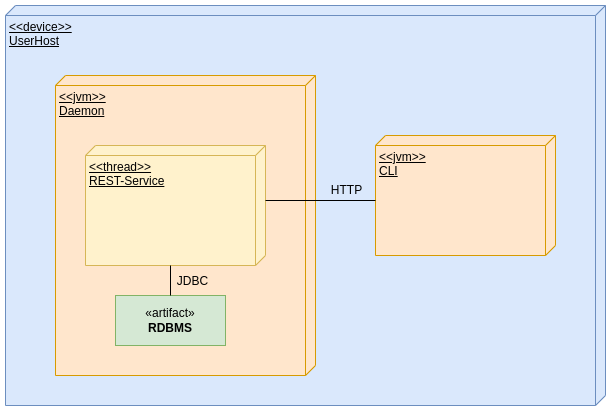
\includegraphics[width=1\textwidth]{assets/DeplDiagram}
        \caption{UML Deploymentdiagramm}
        \label{fig:depl-diag}
    \end{figure}

    Das ganze System befindet sich während der Laufzeit auf dem Host-Gerät des Anwenders.
    Dazu werden zwei separate Jar-Dateien ausgeliefert.
    Die Erste sollte bereits beim Start des Geräts ausgeführt werden und die JVM für den Daemon starten.
    Dieser startet einen Webservice, der REST-Schnittstellen für die Steuerung des Daemons anbietet.
    Dieser REST-Service kommuniziert ausserdem über JDBC mit einem RDBMS, welches in Form von einer einzigen Datei (SQLite)
    in der Daemon-Applikation embedded ist.

    Das zweite Jar sollte dann manuell vom Anwender gestartet werden sobald er Funktionen des Daemons ausführen möchte.
    Dieses Jar startet wiederum eine zweite JVM, welche ein CLI für den Anwender mit bestimmten Kommandos zur Verfügung stellt.
    Diese CLI sendet dann über HTTP die entsprechenden Anfragen an den Daemon, die zur Erfüllung der Anweisungen des Anwenders führen.


    \section{Lizenzierung}


    \section{Installationshandbuch \& Skript}


    \section{Benutzerhandbuch}


    \chapter{Fazit}


    \section{Diskussion}


    \section{Zusammenfassung}


    \section{Zukünftige Arbeiten}
    \url{https://doi.org/10.1145/3664811}


    \chapter{Glossar}


    \chapter{Index}


    \chapter{Bibliografie}


    \chapter{Anhang}


    \section{Facsimile der Projektbeschreibung}


    \section{Erklärung zur Urheberschaft}

\end{document}
